

\tikzset{every picture/.style={line width=0.75pt}} %set default line width to 0.75pt        

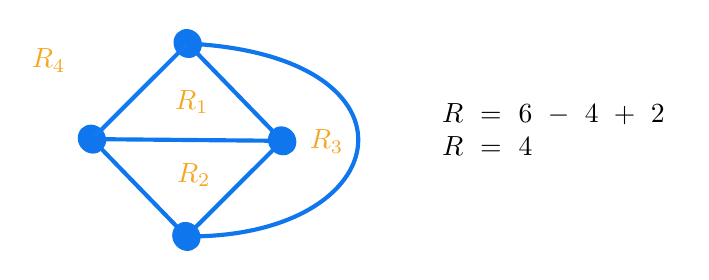
\begin{tikzpicture}[x=0.75pt,y=0.75pt,yscale=-1,xscale=1]
%uncomment if require: \path (0,151); %set diagram left start at 0, and has height of 151

%Shape: Ellipse [id:dp6424091519689461] 
\draw  [draw opacity=0][fill={rgb, 255:red, 15; green, 118; blue, 237 }  ,fill opacity=1 ] (108.4,27.3) .. controls (112.18,27.47) and (115.33,30.72) .. (115.45,34.57) .. controls (115.56,38.42) and (112.59,41.4) .. (108.82,41.23) .. controls (105.04,41.07) and (101.89,37.81) .. (101.77,33.96) .. controls (101.66,30.12) and (104.63,27.13) .. (108.4,27.3) -- cycle ;
%Shape: Ellipse [id:dp4868952713488026] 
\draw  [draw opacity=0][fill={rgb, 255:red, 15; green, 118; blue, 237 }  ,fill opacity=1 ] (62.25,73.36) .. controls (66.03,73.52) and (69.18,76.78) .. (69.29,80.63) .. controls (69.41,84.47) and (66.44,87.45) .. (62.67,87.29) .. controls (58.89,87.12) and (55.74,83.87) .. (55.62,80.02) .. controls (55.51,76.17) and (58.48,73.19) .. (62.25,73.36) -- cycle ;
%Straight Lines [id:da44467552426780155] 
\draw [color={rgb, 255:red, 16; green, 121; blue, 243 }  ,draw opacity=1 ][fill={rgb, 255:red, 0; green, 0; blue, 0 }  ,fill opacity=1 ][line width=1.5]    (108.61,34.27) -- (62.46,80.32) ;
%Shape: Ellipse [id:dp3390874097767833] 
\draw  [draw opacity=0][fill={rgb, 255:red, 15; green, 118; blue, 237 }  ,fill opacity=1 ] (153.91,74.18) .. controls (157.68,74.35) and (160.84,77.61) .. (160.95,81.45) .. controls (161.06,85.3) and (158.1,88.28) .. (154.32,88.11) .. controls (150.55,87.95) and (147.39,84.69) .. (147.28,80.85) .. controls (147.16,77) and (150.13,74.02) .. (153.91,74.18) -- cycle ;
%Shape: Ellipse [id:dp5106914064389432] 
\draw  [draw opacity=0][fill={rgb, 255:red, 15; green, 118; blue, 237 }  ,fill opacity=1 ] (107.76,120.24) .. controls (111.53,120.41) and (114.68,123.66) .. (114.8,127.51) .. controls (114.91,131.35) and (111.94,134.34) .. (108.17,134.17) .. controls (104.39,134) and (101.24,130.75) .. (101.13,126.9) .. controls (101.01,123.05) and (103.98,120.07) .. (107.76,120.24) -- cycle ;
%Straight Lines [id:da763734854884363] 
\draw [color={rgb, 255:red, 15; green, 118; blue, 237 }  ,draw opacity=1 ][fill={rgb, 255:red, 0; green, 0; blue, 0 }  ,fill opacity=1 ][line width=1.5]    (154.11,81.15) -- (107.96,127.2) ;
%Straight Lines [id:da588551383268862] 
\draw [color={rgb, 255:red, 15; green, 118; blue, 237 }  ,draw opacity=1 ][fill={rgb, 255:red, 0; green, 0; blue, 0 }  ,fill opacity=1 ][line width=1.5]    (108.61,34.27) -- (154.11,81.15) ;
%Straight Lines [id:da14849799274214592] 
\draw [color={rgb, 255:red, 15; green, 118; blue, 237 }  ,draw opacity=1 ][fill={rgb, 255:red, 0; green, 0; blue, 0 }  ,fill opacity=1 ][line width=1.5]    (62.46,80.32) -- (107.96,127.2) ;
%Straight Lines [id:da7402882637314507] 
\draw [color={rgb, 255:red, 15; green, 118; blue, 237 }  ,draw opacity=1 ][fill={rgb, 255:red, 0; green, 0; blue, 0 }  ,fill opacity=1 ][line width=1.5]    (154.11,81.15) -- (62.46,80.32) ;
%Curve Lines [id:da2331445702439543] 
\draw [color={rgb, 255:red, 15; green, 118; blue, 237 }  ,draw opacity=1 ][line width=1.5]    (108.61,34.27) .. controls (226.11,40.06) and (210.11,128.06) .. (107.96,127.2) ;

% Text Node
\draw (32,35.4) node [anchor=north west][inner sep=0.75pt]  [color={rgb, 255:red, 245; green, 166; blue, 35 }  ,opacity=1 ]  {$R_{4}$};
% Text Node
\draw (102,90.4) node [anchor=north west][inner sep=0.75pt]  [color={rgb, 255:red, 245; green, 166; blue, 35 }  ,opacity=1 ]  {$R_{2}$};
% Text Node
\draw (166,74.4) node [anchor=north west][inner sep=0.75pt]  [color={rgb, 255:red, 245; green, 166; blue, 35 }  ,opacity=1 ]  {$R_{3}$};
% Text Node
\draw (101,55.4) node [anchor=north west][inner sep=0.75pt]  [color={rgb, 255:red, 245; green, 166; blue, 35 }  ,opacity=1 ]  {$R_{1}$};
% Text Node
\draw (223,59.4) node [anchor=north west][inner sep=0.75pt]  [color={rgb, 255:red, 0; green, 0; blue, 0 }  ,opacity=1 ]  {$ \begin{array}{l}
R\ =\ 6\ -\ 4\ +\ 2\\
R\ =\ 4
\end{array}$};


\end{tikzpicture}